% REMEMBER: You must not plagiarise anything in your report. Be extremely careful.

\documentclass{l4proj}

    
%
% put any additional packages here
%

\begin{document}

%==============================================================================
%% METADATA
\title{Level 4 Project Report Template}
\author{John H. Williamson}
\date{September 14, 2018}

\maketitle

%==============================================================================
%% ABSTRACT
\begin{abstract}
    Every abstract follows a similar pattern. Motivate; set aims; describe work; explain results.
    \vskip 0.5em
    ``XYZ is bad. This project investigated ABC to determine if it was better. 
    ABC used XXX and YYY to implement ZZZ. This is particularly interesting as XXX and YYY have
    never been used together. It was found that  
    ABC was 20\% better than XYZ, though it caused rabies in half of subjects.''
\end{abstract}

%==============================================================================

% EDUCATION REUSE CONSENT FORM
% If you consent to your project being shown to future students for educational purposes
% then insert your name and the date below to  sign the education use form that appears in the front of the document. 
% You must explicitly give consent if you wish to do so.
% If you sign, your project may be included in the Hall of Fame if it scores particularly highly.
%
% Please note that you are under no obligation to sign 
% this declaration, but doing so would help future students.
%
%\def\consentname {My Name} % your full name
%\def\consentdate {20 March 2018} % the date you agree
%
\educationalconsent


%==============================================================================
\tableofcontents

%==============================================================================
%% Notes on formatting
%==============================================================================
% The first page, abstract and table of contents are numbered using Roman numerals and are not
% included in the page count. 
%
% From now on pages are numbered
% using Arabic numerals. Therefore, immediately after the first call to \chapter we need the call
% \pagenumbering{arabic} and this should be called once only in the document. 
%
% Do not alter the bibliography style.
%
% The first Chapter should then be on page 1. You are allowed 40 pages for a 40 credit project and 30 pages for a 
% 20 credit report. This includes everything numbered in Arabic numerals (excluding front matter) up
% to but excluding the appendices and bibliography.
%
% You must not alter text size (it is currently 10pt) or alter margins or spacing.
%
%
%==================================================================================================================================
%
% IMPORTANT
% The chapter headings here are **suggestions**. You don't have to follow this model if
% it doesn't fit your project. Every project should have an introduction and conclusion,
% however. 
%
%==================================================================================================================================
\chapter{Introduction}

% reset page numbering. Don't remove this!
\pagenumbering{arabic} 


\section{Concurrency and Distributed Systems}

Concurrency and distributed systems are becoming increasingly important in modern computational science, especially in the context of cloud computing and big data. Sutter and Larus (2005) emphasize that with the proliferation of multicore processors, the software industry needs to adopt new tools and ways of thinking in order to fully utilize the potential of multicore processors. Concurrency refers to the ability of a system to handle multiple tasks at the same time, which allows efficient use of computational resources. For example, by processing hundreds or even thousands of client requests in parallel, modern Web servers are able to dramatically improve response times and system throughput. This shift in demand requires mainstream software development to stop ignoring concurrency, a challenge that requires developers to master the design and implementation of concurrent programs (Sutter & Larus, 2005).
    
The design of Multiplayer Online Role-Playing Game (MMORPG) servers, such as exemplified by the World of Warcraft (Figure \ref{fig:WoWlogo}) demonstrates the value of concurrent programming in real-world applications, where the use of a client-server model and event-driven architecture enables asynchronous processing of player requests. Kim and Kim's (2019) study, by utilizing Input/Output Completion Port (IOCP) and multithreading techniques, has demonstrated methods to effectively improve server performance, handle concurrent connections and employ fine-grained locking mechanisms for access control of shared resources to reduce the risk of deadlock and effectively improve system responsiveness and throughput.

\begin{figure}[h]
    \centering
    \begin{minipage}[t]{0.35\textwidth}
        \centering
        
\includegraphics[width=\linewidth,height=5cm,keepaspectratio]{images/WoWlogo.png}
        \caption{World of Warcraft}
        \label{fig:WoWlogo}
    \end{minipage}
    \quad
    \begin{minipage}[t]{0.30\textwidth}
        \centering
        \includegraphics[width=\linewidth,height=5cm,keepaspectratio]{images/PokemonGo.jpeg}
        \caption{Pokemon GO}
        \label{fig:PokemonGo}
    \end{minipage}
\end{figure}

On the other hand, Distributed systems achieve workload decentralization by assigning tasks across multiple compute nodes, which is especially critical for processing large-scale data sets. For example, Google's Bigtable and Apache Hadoop's Distributed File System (HDFS) are capable of handling petabytes of data and supporting complex data analysis tasks. In this context, the distributed architecture of Pokemon GO(Figure \ref{fig:PokemonGo}) demonstrates the efficient ability of distributed systems to manage and synchronize millions of players globally, through a network of servers deployed in multiple locations around the world, and the use of geo-distributed database technology to decentralize the storage of data based on the geographic location of players, showing the importance of this technology in dealing with large-scale, real-time interactive applications.
		
The combination of concurrency and distributed systems not only greatly improves the efficiency of task processing, but also enhances the reliability and scalability of the system. In the case of distributed databases, for example, data is replicated across multiple nodes, ensuring that the entire system can maintain normal operation even if some of the nodes fail. In addition, this technology supports the dynamic adjustment of computing resources according to actual demand, a feature that is widely used in cloud service platforms such as Amazon Web Services and Microsoft Azure. This exposition not only demonstrates the key role of concurrent programming in ensuring high availability and optimizing user experience, but also provides an important reference for designing efficient concurrent and distributed systems.

\section{Challenges}

While these systems are capable of handling unprecedented amounts of data and computational tasks, they also introduce a new set of challenges. 

\subsection{Thread Deadlock}

A commonly faced problem in concurrent programming is thread deadlock, a situation where multiple threads are unable to move forward because they are waiting for each other to release resources. As an example, a deadlock is caused when two threads each have some resources locked and are both waiting for the other to release the resources they hold. This situation is particularly common in database transaction processing and operating system resource allocation, and seriously affects the stability and efficiency of the programme.


\subsection{Communication Mismatch}

Communication mismatch is another critical issue in distributed systems. Nodes in a distributed environment need to exchange information frequently, and any inconsistency in communication protocols or data formats can lead to major failures. Taking microservice architecture as an example, if the communication interfaces between services are not clearly defined or fail to maintain compatibility during version updates, it may lead to the functional failure of the whole system. This is particularly noticeable in fast iterative and multi-team projects and requires special attention.

\section{Research Goals}

The aim of this research is to develop a runtime environment generator specifically designed to support a new programming language, the Pat language.The Pat language addresses the programming challenges of concurrency and distributed systems, and by introducing advanced concurrent programming primitives and a unique mailbox type system, it aims to provide developers with a more intuitive and concise way to handle concurrent tasks and communication flows. While a type checker for the Pat language has been implemented, an efficient execution environment has yet to be developed. The main goal of this project is to build such an execution environment so that developers can easily write, test and run programmes written in the Pat language.

This runtime environment generator should not only satisfy the runtime requirements of a general programming language, such as memory management and exception handling, but should also focus on the specific needs of concurrent and distributed computing. By providing such a tool, the Pat language will become a powerful support for the research and development of concurrent and distributed systems, which not only promotes the wide application and continuous development of the Pat language, but also provides new perspectives and methods for exploring problems in the field of concurrent programming, and establishes a solid foundation for future technological innovations.


%==================================================================================================================================
\chapter{Background}

\section{Concurrency}
Modern concurrent programming uses two main paradigms: Message-Passing Concurrency and Shared-Memory Concurrency, which use different strategies and mechanisms to handle concurrent tasks.

\subsection{Shared Memory}
Shared-memory concurrency model allows multiple processes or threads to share the same memory space and communicate through this shared space. While this approach improves efficiency in certain scenarios, it also introduces data consistency and synchronisation issues. In the shared memory model, developers must carefully handle locking mechanisms and synchronisation issues to prevent deadlocks and race conditions from occurring.Java and C++ are examples of languages that support this concurrency model.

\subsection{Message Passing}
In contrast, Message-passing Concurrency is a programming paradigm that enables communication and coordination by sending and receiving messages between processes or threads. The main advantage of this approach is that it provides a clear mechanism to avoid data contention and conflict, as data is passed through message exchange rather than sharing. In this model, each process or thread has a separate memory space and all communication takes place through well-defined message interfaces, but additional overhead is introduced[5].The Erlang language and the Akka framework are excellent representatives of this model.

Although message-passing concurrency and shared-memory concurrency each have their own strengths, message-passing concurrency provides a clearer and more controlled approach to dealing with the problems of distributed systems and reducing complex synchronisation issues. Therefore, the message-passing concurrency paradigm was chosen in the design of the Pat language in order to provide a safer and more intuitive approach to concurrent programming.

\section{Communication Mechanisms}
With its clear communication mechanism, the message-passing concurrency model provides the Pat language with an effective means to avoid data conflicts and competition, which significantly enhances the advantages of concurrent program design. On this basis, by introducing two high-level abstractions, Channel and Actors, not only the expressive ability of message-passing concurrency is further enhanced, but also the manageability and extensibility of concurrent programs are significantly improved (Figure \ref{fig:channel_actor}). Nevertheless, both models have revealed some problems in practice.

\subsection{Channel}
The Channels model, typically found in languages such as Go, implements inter-process communication through named channels, as depicted in Figure \ref{fig:channel_actor}.a. Processes or threads communicate and coordinate with each other by passing messages through these named channels.The main advantage of Channels is their flexibility and simple type system, which makes the model easy to understand and deploy, especially in situations where communication patterns change frequently. However, Channels can raise complex synchronisation issues, such as data contention and deadlocks when multiple processes access the same channel at the same time without proper synchronisation mechanisms.

\subsection{Actor}
The Actors model, as opposed to Channels, is implemented in Erlang or Elixir, where each Actor acts as an addressable process with a single message queue or mailbox for receiving messages (Figure \ref{fig:channel_actor}.b). Each Actor acts as an independent entity and interacts with each other through asynchronous message passing.The strength of the Actors model lies in its natural support for distributed computing, especially in terms of fault tolerance and system reliability. The independence of each Actor makes the model particularly suitable for building large-scale, scalable distributed applications. However, the Actors model faces its own challenges, especially in message management. Since each Actor's mailbox may receive any type of message, runtime errors may be raised, such as receiving a message type that cannot be processed. In addition, performance may become problematic when managing a large number of fine-grained Actors, especially in application scenarios that require fast response and efficient processing of a large number of messages.

\begin{figure}
    \centering
    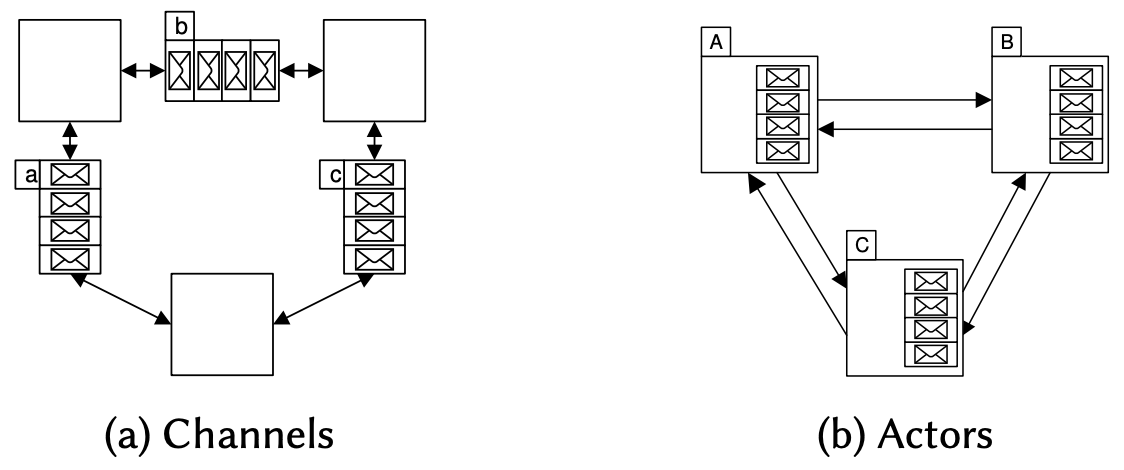
\includegraphics[width=0.7\linewidth]{images/channel_actor.png}    
    \caption{ (a) illustrates the Channels model with concurrent units communicating via message-passing channels. (b) shows the Actors model where each Actor independently processes messages from its queue. (Fowler et al. 2017)
    }
    \label{fig:channel_actor} 
\end{figure}

\subsection{Pat's Solution}
To cope with these challenges, the introduction of Actor type systems has become an important advancement. In this context, the design of the Pat language introduces a new solution based on the Actor model along with a mailbox behavioural type system for the first time in a behavioural type system at the programming language level.


\section{Behavioural Type System}
Behavioural type system is a type system used in the field of concurrent and distributed programming to describe and manage system behaviour. This type system not only contains information about the type of data, but also extends to the description of program behaviour, such as message passing, inter-process communication patterns and protocol constraints. The core purpose of a behavioural type system is to improve the reliability and security of concurrent programs. By checking the behavioural patterns of a program at compile time, a behavioural type system ensures the correctness and stability of the program at runtime.

\subsection{Mailbox Type}
Mailbox types, a key part of the behavioural type system, were initially used in process algorithms to capture mainly mailbox contents as exchange regular expressions. Introduced by Ugo de'Liguoro and Luca Padovani in 2018 [3], they are intended to enhance the message-passing mechanism of programming languages based on the actor model. Mailbox types specify type annotations for each actor's mailbox, which define not only the types of messages that the mailbox can receive, but also detail expected behaviour patterns such as the order in which messages are sent and received. This careful type annotation enables strict checking of message delivery patterns, thus enabling precise control of complex communication behaviour and significant improvements in type safety in concurrent programming, avoiding problems such as protocol violations and deadlocks. The application of mailbox types, an innovative practice in the Pat language, brings significant improvements to the security and robustness of concurrent programs, opening up new perspectives and solutions in the field of concurrent programming.


\section{Scheduling}
Scheduling in computing systems refers to the strategic scheduling and management of the order in which jobs are executed. This process is a high-level strategic decision making aimed at optimising processes and computational tasks in terms of time and resource allocation. In a concurrent environment, it is the responsibility of the scheduler to determine the timing of execution of each task to ensure that processor resources are used efficiently while minimising the task completion time. In distributed systems, the scheduler's responsibility extends to task allocation across different compute nodes, aiming to maximise the utilisation efficiency of each node in the network. Regardless of the type of system, the fundamental purpose of scheduling is to improve the overall throughput capacity of the system. In this framework, control flow management techniques, such as CPS and CEK, provide execution-level support and implementation mechanisms for scheduling, enabling scheduling policies to be applied more flexibly and efficiently to complex computing tasks and system architectures.

\subsection{CPS and CEK}
Continuation Passing Style (CPS) is a high-level control flow management technique that operates by explicitly passing the unexecuted portion of a program, called a "continuation". In the functional programming paradigm, this approach allows a function not to return a result directly, but to continue execution by accepting another function (i.e., a "continue") and passing it control. This style is inherently suited to implementing non-blocking and asynchronous operations, and provides a great deal of flexibility in modern programming. Although CPS elegantly handles asynchronicity and non-blocking operations, it introduces the need for concurrent multi-process control and complex communication patterns in concurrent and distributed system applications. However, CPS applications may make the code structure appear more complex and rigid, which not only challenges the readability of the programme but also increases the maintenance cost.

The Pat language, however, is dedicated to the problem of communication in concurrent and distributed systems, employing mailbox types as its core communication mechanism. In such systems, the communication process is often asynchronous, the order in which messages are delivered is uncertain, and multiple concurrent senders and receivers may be involved. In contrast to CPS, CEK-style abstract machines provide a more detailed division of programme state - Continuation, Environment and Control - through more detailed Explicit management provides a more structured and flexible framework for dealing with such complex communications. In the context of Pat language applications, where nested evaluation contexts and aliasing issues need to be considered, the CEK model demonstrates excellent adaptability and handling capabilities, making it ideal for supporting the features of the Pat language.

\section{Implementing Pat in OCaml}
The tool for implementing the Pat language is the use of the OCaml language. Because of its excellent functional programming features, powerful type system and pattern matching capabilities, these advantages make OCaml particularly suitable for developing compilers and dealing with concurrency. Compared to other programming languages, OCaml provides a more efficient and secure programming environment, showing its unique advantages especially in handling complex communications in concurrent and distributed systems.


%==================================================================================================================================
\chapter{Analysis/Requirements}
What is the problem that you want to solve, and how did you arrive at it?
\section{Guidance}
Make it clear how you derived the constrained form of your problem via a clear and logical process. 

%==================================================================================================================================
\chapter{Design}
How is this problem to be approached, without reference to specific implementation details? 
\section{Guidance}
Design should cover the abstract design in such a way that someone else might be able to do what you did, but with a different language or library or tool.

%==================================================================================================================================
\chapter{Implementation}
What did you do to implement this idea, and what technical achievements did you make?
\section{Guidance}
You can't talk about everything. Cover the high level first, then cover important, relevant or impressive details.



\section{General points}

These points apply to the whole dissertation, not just this chapter.



\subsection{Figures}
\emph{Always} refer to figures included, like Figure \ref{fig:relu}, in the body of the text. Include full, explanatory captions and make sure the figures look good on the page.
You may include multiple figures in one float, as in Figure \ref{fig:synthetic}, using \texttt{subcaption}, which is enabled in the template.



% Figures are important. Use them well.
\begin{figure}
    \centering
    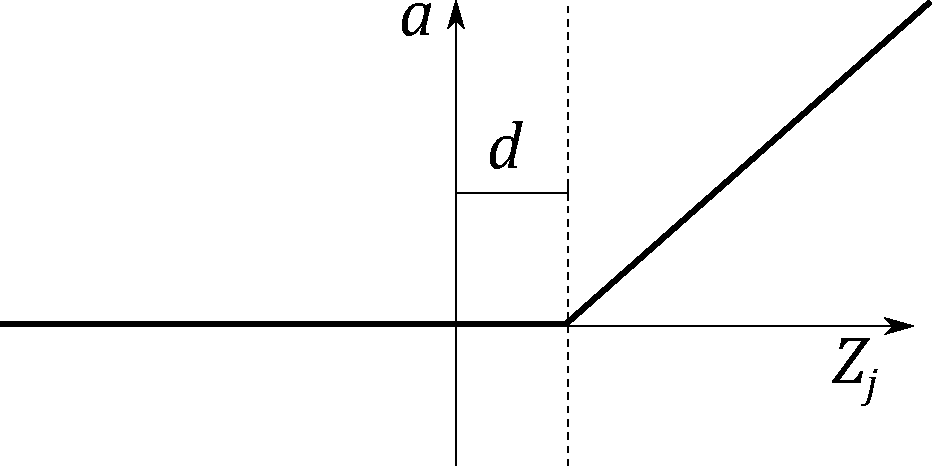
\includegraphics[width=0.5\linewidth]{images/relu.pdf}    

    \caption{In figure captions, explain what the reader is looking at: ``A schematic of the rectifying linear unit, where $a$ is the output amplitude,
    $d$ is a configurable dead-zone, and $Z_j$ is the input signal'', as well as why the reader is looking at this: 
    ``It is notable that there is no activation \emph{at all} below 0, which explains our initial results.'' 
    \textbf{Use vector image formats (.pdf) where possible}. Size figures appropriately, and do not make them over-large or too small to read.
    }

    % use the notation fig:name to cross reference a figure
    \label{fig:relu} 
\end{figure}


\begin{figure}
    \centering
    \begin{subfigure}[b]{0.45\textwidth}
        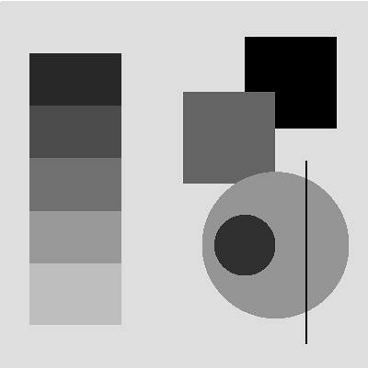
\includegraphics[width=\textwidth]{images/synthetic.png}
        \caption{Synthetic image, black on white.}
        \label{fig:syn1}
    \end{subfigure}
    ~ %add desired spacing between images, e. g. ~, \quad, \qquad, \hfill etc. 
      %(or a blank line to force the subfigure onto a new line)
    \begin{subfigure}[b]{0.45\textwidth}
        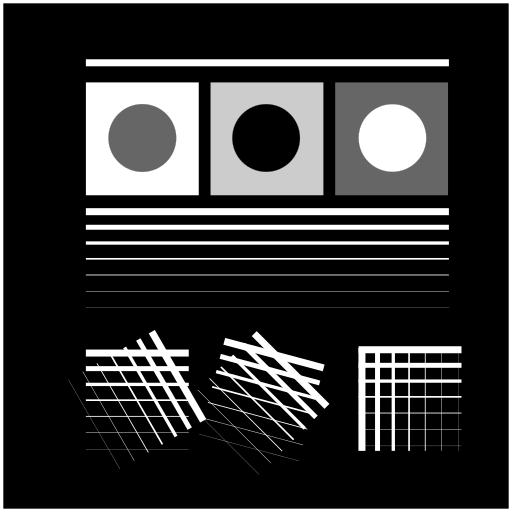
\includegraphics[width=\textwidth]{images/synthetic_2.png}
        \caption{Synthetic image, white on black.}
        \label{fig:syn2}
    \end{subfigure}
    ~ %add desired spacing between images, e. g. ~, \quad, \qquad, \hfill etc. 
    %(or a blank line to force the subfigure onto a new line)    
    \caption{Synthetic test images for edge detection algorithms. \subref{fig:syn1} shows various gray levels that require an adaptive algorithm. \subref{fig:syn2}
    shows more challenging edge detection tests that have crossing lines. Fusing these into full segments typically requires algorithms like the Hough transform.
    This is an example of using subfigures, with \texttt{subref}s in the caption.
    }\label{fig:synthetic}
\end{figure}

\clearpage

\subsection{Equations}

Equations should be typeset correctly and precisely. Make sure you get parenthesis sizing correct, and punctuate equations correctly 
(the comma is important and goes \textit{inside} the equation block). Explain any symbols used clearly if not defined earlier. 

For example, we might define:
\begin{equation}
    \hat{f}(\xi) = \frac{1}{2}\left[ \int_{-\infty}^{\infty} f(x) e^{2\pi i x \xi} \right],
\end{equation}    
where $\hat{f}(\xi)$ is the Fourier transform of the time domain signal $f(x)$.

\subsection{Algorithms}
Algorithms can be set using \texttt{algorithm2e}, as in Algorithm \ref{alg:metropolis}.

% NOTE: line ends are denoted by \; in algorithm2e
\begin{algorithm}
    \DontPrintSemicolon
    \KwData{$f_X(x)$, a probability density function returing the density at $x$.\; $\sigma$ a standard deviation specifying the spread of the proposal distribution.\;
    $x_0$, an initial starting condition.}
    \KwResult{$s=[x_1, x_2, \dots, x_n]$, $n$ samples approximately drawn from a distribution with PDF $f_X(x)$.}
    \Begin{
        $s \longleftarrow []$\;
        $p \longleftarrow f_X(x)$\;
        $i \longleftarrow 0$\;
        \While{$i < n$}
        {
            $x^\prime \longleftarrow \mathcal{N}(x, \sigma^2)$\;
            $p^\prime \longleftarrow f_X(x^\prime)$\;
            $a \longleftarrow \frac{p^\prime}{p}$\;
            $r \longleftarrow U(0,1)$\;
            \If{$r<a$}
            {
                $x \longleftarrow x^\prime$\;
                $p \longleftarrow f_X(x)$\;
                $i \longleftarrow i+1$\;
                append $x$ to $s$\;
            }
        }
    }
    
\caption{The Metropolis-Hastings MCMC algorithm for drawing samples from arbitrary probability distributions, 
specialised for normal proposal distributions $q(x^\prime|x) = \mathcal{N}(x, \sigma^2)$. The symmetry of the normal distribution means the acceptance rule takes the simplified form.}\label{alg:metropolis}
\end{algorithm}

\subsection{Tables}

If you need to include tables, like Table \ref{tab:operators}, use a tool like https://www.tablesgenerator.com/ to generate the table as it is
extremely tedious otherwise. 

\begin{table}[]
    \caption{The standard table of operators in Python, along with their functional equivalents from the \texttt{operator} package. Note that table
    captions go above the table, not below. Do not add additional rules/lines to tables. }\label{tab:operators}
    %\tt 
    \rowcolors{2}{}{gray!3}
    \begin{tabular}{@{}lll@{}}
    %\toprule
    \textbf{Operation}    & \textbf{Syntax}                & \textbf{Function}                            \\ %\midrule % optional rule for header
    Addition              & \texttt{a + b}                          & \texttt{add(a, b)}                                    \\
    Concatenation         & \texttt{seq1 + seq2}                    & \texttt{concat(seq1, seq2)}                           \\
    Containment Test      & \texttt{obj in seq}                     & \texttt{contains(seq, obj)}                           \\
    Division              & \texttt{a / b}                          & \texttt{div(a, b) }  \\
    Division              & \texttt{a / b}                          & \texttt{truediv(a, b) } \\
    Division              & \texttt{a // b}                         & \texttt{floordiv(a, b)}                               \\
    Bitwise And           & \texttt{a \& b}                         & \texttt{and\_(a, b)}                                  \\
    Bitwise Exclusive Or  & \texttt{a \textasciicircum b}           & \texttt{xor(a, b)}                                    \\
    Bitwise Inversion     & \texttt{$\sim$a}                        & \texttt{invert(a)}                                    \\
    Bitwise Or            & \texttt{a | b}                          & \texttt{or\_(a, b)}                                   \\
    Exponentiation        & \texttt{a ** b}                         & \texttt{pow(a, b)}                                    \\
    Identity              & \texttt{a is b}                         & \texttt{is\_(a, b)}                                   \\
    Identity              & \texttt{a is not b}                     & \texttt{is\_not(a, b)}                                \\
    Indexed Assignment    & \texttt{obj{[}k{]} = v}                 & \texttt{setitem(obj, k, v)}                           \\
    Indexed Deletion      & \texttt{del obj{[}k{]}}                 & \texttt{delitem(obj, k)}                              \\
    Indexing              & \texttt{obj{[}k{]}}                     & \texttt{getitem(obj, k)}                              \\
    Left Shift            & \texttt{a \textless{}\textless b}       & \texttt{lshift(a, b)}                                 \\
    Modulo                & \texttt{a \% b}                         & \texttt{mod(a, b)}                                    \\
    Multiplication        & \texttt{a * b}                          & \texttt{mul(a, b)}                                    \\
    Negation (Arithmetic) & \texttt{- a}                            & \texttt{neg(a)}                                       \\
    Negation (Logical)    & \texttt{not a}                          & \texttt{not\_(a)}                                     \\
    Positive              & \texttt{+ a}                            & \texttt{pos(a)}                                       \\
    Right Shift           & \texttt{a \textgreater{}\textgreater b} & \texttt{rshift(a, b)}                                 \\
    Sequence Repetition   & \texttt{seq * i}                        & \texttt{repeat(seq, i)}                               \\
    Slice Assignment      & \texttt{seq{[}i:j{]} = values}          & \texttt{setitem(seq, slice(i, j), values)}            \\
    Slice Deletion        & \texttt{del seq{[}i:j{]}}               & \texttt{delitem(seq, slice(i, j))}                    \\
    Slicing               & \texttt{seq{[}i:j{]}}                   & \texttt{getitem(seq, slice(i, j))}                    \\
    String Formatting     & \texttt{s \% obj}                       & \texttt{mod(s, obj)}                                  \\
    Subtraction           & \texttt{a - b}                          & \texttt{sub(a, b)}                                    \\
    Truth Test            & \texttt{obj}                            & \texttt{truth(obj)}                                   \\
    Ordering              & \texttt{a \textless b}                  & \texttt{lt(a, b)}                                     \\
    Ordering              & \texttt{a \textless{}= b}               & \texttt{le(a, b)}                                     \\
    % \bottomrule
    \end{tabular}
    \end{table}
\subsection{Code}

Avoid putting large blocks of code in the report (more than a page in one block, for example). Use syntax highlighting if possible, as in Listing \ref{lst:callahan}.

\begin{lstlisting}[language=python, float, caption={The algorithm for packing the $3\times 3$ outer-totalistic binary CA successor rule into a 
    $16\times 16\times 16\times 16$ 4 bit lookup table, running an equivalent, notionally 16-state $2\times 2$ CA.}, label=lst:callahan]
    def create_callahan_table(rule="b3s23"):
        """Generate the lookup table for the cells."""        
        s_table = np.zeros((16, 16, 16, 16), dtype=np.uint8)
        birth, survive = parse_rule(rule)

        # generate all 16 bit strings
        for iv in range(65536):
            bv = [(iv >> z) & 1 for z in range(16)]
            a, b, c, d, e, f, g, h, i, j, k, l, m, n, o, p = bv

            # compute next state of the inner 2x2
            nw = apply_rule(f, a, b, c, e, g, i, j, k)
            ne = apply_rule(g, b, c, d, f, h, j, k, l)
            sw = apply_rule(j, e, f, g, i, k, m, n, o)
            se = apply_rule(k, f, g, h, j, l, n, o, p)

            # compute the index of this 4x4
            nw_code = a | (b << 1) | (e << 2) | (f << 3)
            ne_code = c | (d << 1) | (g << 2) | (h << 3)
            sw_code = i | (j << 1) | (m << 2) | (n << 3)
            se_code = k | (l << 1) | (o << 2) | (p << 3)

            # compute the state for the 2x2
            next_code = nw | (ne << 1) | (sw << 2) | (se << 3)

            # get the 4x4 index, and write into the table
            s_table[nw_code, ne_code, sw_code, se_code] = next_code

        return s_table

\end{lstlisting}

%==================================================================================================================================
\chapter{Evaluation} 
How good is your solution? How well did you solve the general problem, and what evidence do you have to support that?

\section{Guidance}
\begin{itemize}
    \item
        Ask specific questions that address the general problem.
    \item
        Answer them with precise evidence (graphs, numbers, statistical
        analysis, qualitative analysis).
    \item
        Be fair and be scientific.
    \item
        The key thing is to show that you know how to evaluate your work, not
        that your work is the most amazing product ever.
\end{itemize}

\section{Evidence}
Make sure you present your evidence well. Use appropriate visualisations, reporting techniques and statistical analysis, as appropriate.

If you visualise, follow the basic rules, as illustrated in Figure \ref{fig:boxplot}:
\begin{itemize}
\item Label everything correctly (axis, title, units).
\item Caption thoroughly.
\item Reference in text.
\item \textbf{Include appropriate display of uncertainty (e.g. error bars, Box plot)}
\item Minimize clutter.
\end{itemize}

See the file \texttt{guide\_to\_visualising.pdf} for further information and guidance.

\begin{figure}
    \centering
    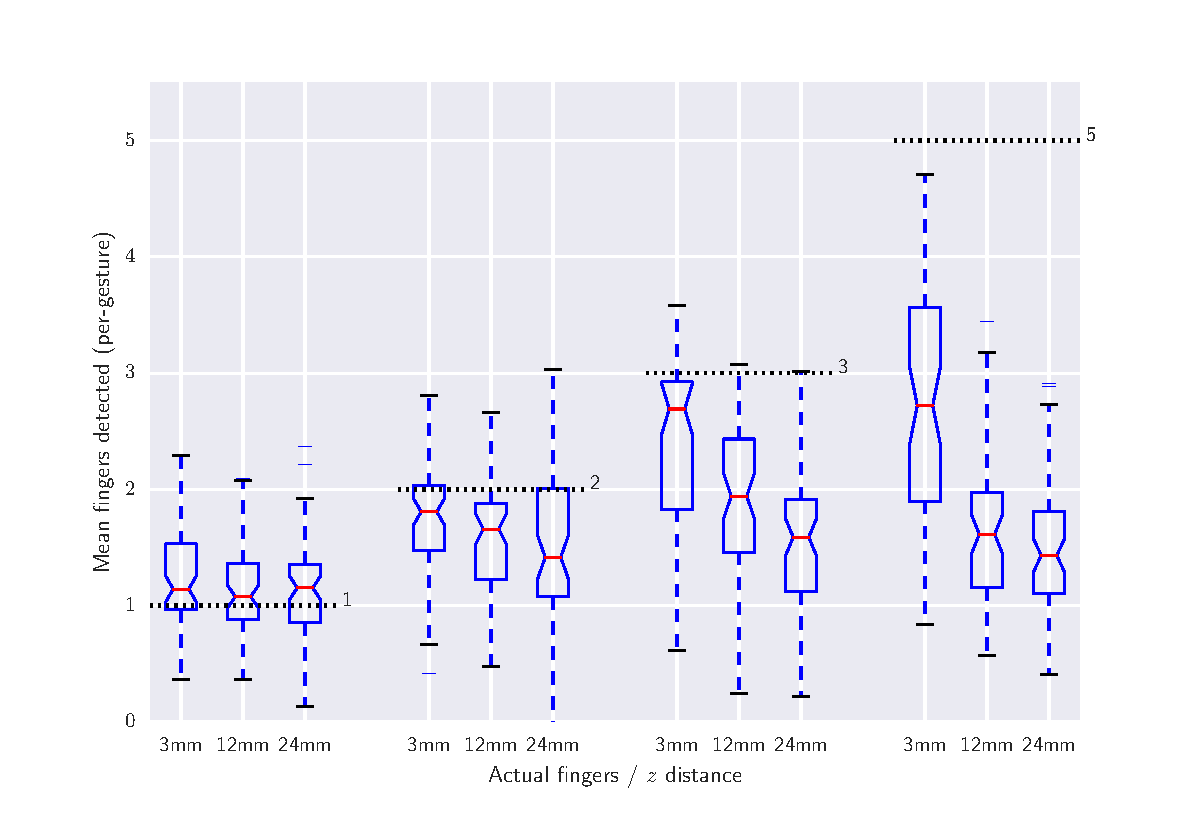
\includegraphics[width=1.0\linewidth]{images/boxplot_finger_distance.pdf}    

    \caption{Average number of fingers detected by the touch sensor at different heights above the surface, averaged over all gestures. Dashed lines indicate
    the true number of fingers present. The Box plots include bootstrapped uncertainty notches for the median. It is clear that the device is biased toward 
    undercounting fingers, particularly at higher $z$ distances.
    }

    % use the notation fig:name to cross reference a figure
    \label{fig:boxplot} 
\end{figure}


%==================================================================================================================================
\chapter{Conclusion}    
Summarise the whole project for a lazy reader who didn't read the rest (e.g. a prize-awarding committee).
\section{Guidance}
\begin{itemize}
    \item
        Summarise briefly and fairly.
    \item
        You should be addressing the general problem you introduced in the
        Introduction.        
    \item
        Include summary of concrete results (``the new compiler ran 2x
        faster'')
    \item
        Indicate what future work could be done, but remember: \textbf{you
        won't get credit for things you haven't done}.
\end{itemize}

%==================================================================================================================================
%
% 
%==================================================================================================================================
%  APPENDICES  

\begin{appendices}

\chapter{Appendices}

Typical inclusions in the appendices are:

\begin{itemize}
\item
  Copies of ethics approvals (required if obtained)
\item
  Copies of questionnaires etc. used to gather data from subjects.
\item
  Extensive tables or figures that are too bulky to fit in the main body of
  the report, particularly ones that are repetitive and summarised in the body.

\item Outline of the source code (e.g. directory structure), or other architecture documentation like class diagrams.

\item User manuals, and any guides to starting/running the software.

\end{itemize}

\textbf{Don't include your source code in the appendices}. It will be
submitted separately.

\end{appendices}

%==================================================================================================================================
%   BIBLIOGRAPHY   

% The bibliography style is abbrvnat
% The bibliography always appears last, after the appendices.

\bibliographystyle{abbrvnat}

\bibliography{l4proj}

\end{document}
